\documentclass{beamer}
\usepackage{beamerthemesplit} % kam neu dazu
\usepackage[utf8]{inputenc}
\usepackage[T1]{fontenc}
\usepackage[ngerman]{babel}



\begin{document}
\title{Mößbauereffekt} 
\author{Paul Kremser, Tobias Grussenemyer}
\date{Versuchsdurchführung: 1. bis 12. März 2010} 

\frame{\titlepage} 

\frame{\frametitle{Inhaltsverzeichnis}\tableofcontents} 

\section{Einleitung}
\subsection{Historisches}
\subsection{Anwendungen}

\frame{\frametitle{Rudolf Mößbauer}
Er ging davon aus, dass sich zwei Quanten die auf diese Weise wechselwirken mit der doppelten Rückstoßgeschwindigkeit aufeinander zu bewegen müssten.
Diese Theorie folgt direkt aus der Impulserhaltung und schien zunächst auch durch das Experiment bestätigt zu werden. Zuerst untersuchte Mössbauer nämlich die
Resonanzabsorption bei Zimmertemperatur und darüber. Als er aber begann Quelle und Absorber abzukühlen, stieg die Intensität des Messsignals plötzlich steil an,
und zwar über die bei hohen Temperaturen gemessene.
}

\section{Theorie und Aufbau}
\subsection{Emission und Absorption}
\begin{enumerate}
 \item Geht ein 
 \item Energieeichung des MCA mit Hilfe eines Americium Strahlers und verschiedener metallischer Floureszenzplättchen (Aufbau mit Drehscheibe)
 \item Mit dem SCA ein Fenster auf die 14,4 KeV Linie setzen.
 \item Mit Hilfe verschiedener Aluminiumplättchen sollen Untergrundmessungen bei verschiedenen Dicken gemacht werden um später auf die Dicke Null extrapolieren zu können.
 \item Aufnahme der Spektren des Einlinien- (Eisen) Absorbers und des 6-Linien- (Edelstahl) Absorbers.
\end{enumerate}
\subsection{Hyperfeinstruktur}

\subsection{Rückstoßfreie Resonanzabsorbtion}

\subsection{Aufbau}


\frame{\frametitle{Resonanzabsorption}
\begin{itemize}
 \item Beim Kernübergang von angeregtem- in Grundzustand
 \item wird ein Photon erzeugt $E_\gamma \approx E_a - E_g$
 \item dieses kann einen anderen Kern anregen
 \item Resonanzabsorption: Gleiche angeregte Zustände
 \item Aus der Impulserhaltung folgt ein Engergiefehlbetrag der doppelten Rückstoßenergie
\end{itemize}
}

\frame{\frametitle{Energieverschiebung}
\begin{figure}
 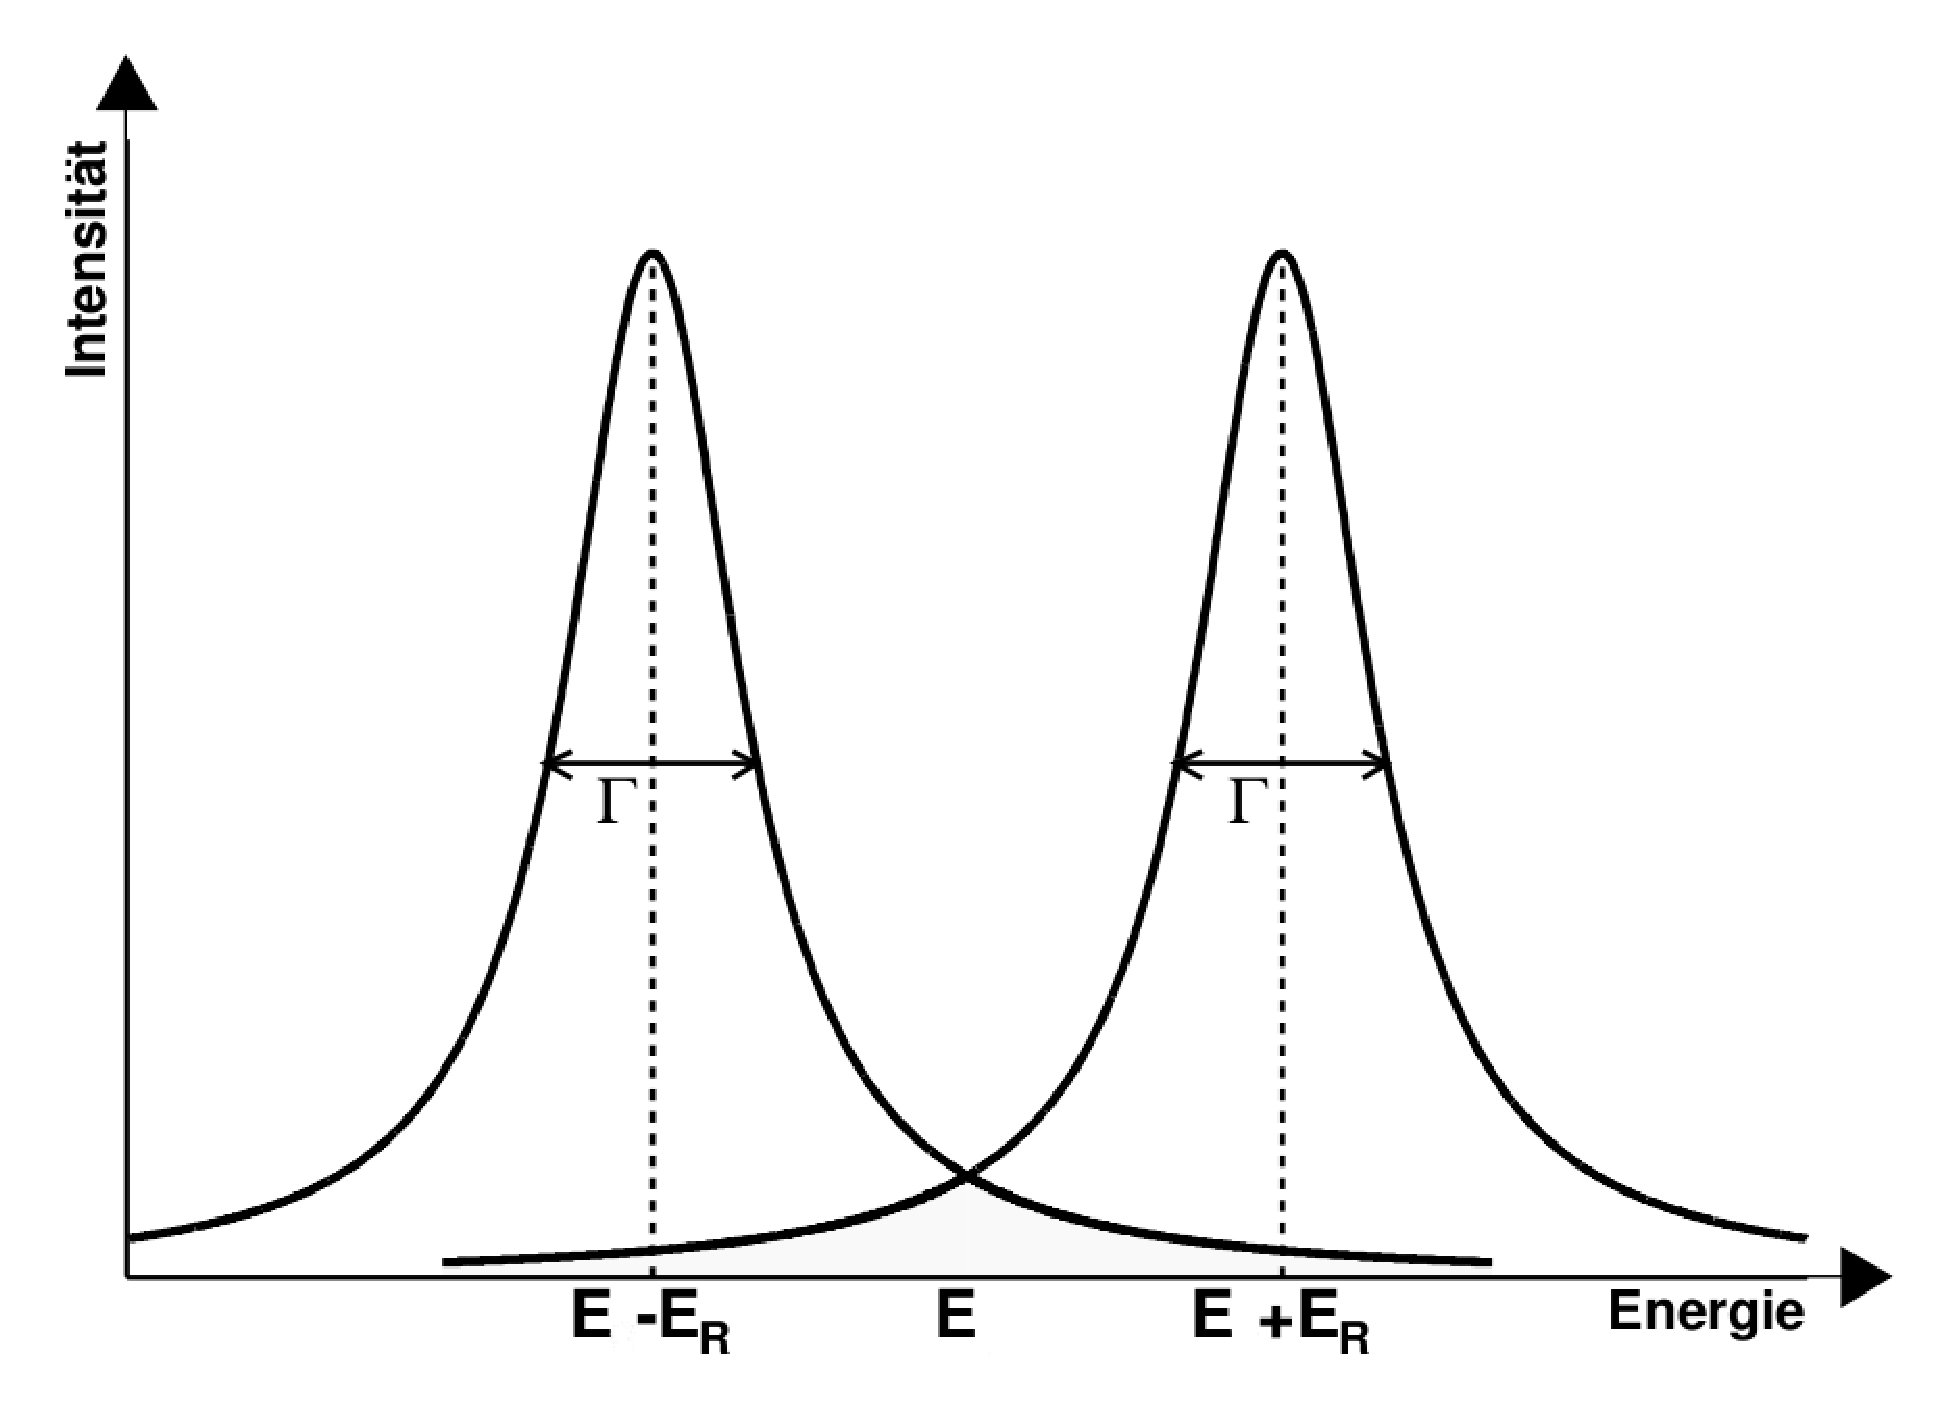
\includegraphics[width=0.7\linewidth]{pictures/energieverschiebung.eps}
 \caption{Energieverschiebung von Emissions- und Absorptionslinie}
 \label{energieverschiebung}
\end{figure}
}

\frame{\frametitle{Debye-Waller-Faktor}
Wie schon erwähnt kann es aber auch vorkommen, dass keine rückstoßfreie Resonanzabsorption auftritt da bei der Absorption oder Emission Gitterschwingungen (Phononen) 
angeregt werden können und somit dem Photon doch wieder nicht die volle Energie des Übergangs zur Verfügung steht. Der Debye-Waller-Faktor $f$ gibt an wie viel rückstoßfreie Resonanzabsorption
auftritt. Er hängt von der Temperatur und der Übergangsenergie ab:
}
\frame{\frametitle{Debye-Waller-Faktor}
\begin{align}
 f = exp\left[ -\frac{3E_R}{2k_B\Theta}\left(1+\left(\frac{2T}{\Theta}\right)^2 \int\limits_{0}^{\frac{\Theta}{T}} \frac{x~dx}{e^x - 1}\right)\right]
\end{align}
und lässt sich für kleine Temperaturen $(T<<\Theta)$ und Kerne im arteigenen kubischen Gitter annähern durch:
\begin{align}
 f \approx exp \left[ -\frac{E_R}{k_B\Theta}\left(\frac{3}{2} + \left(\frac{\pi T}{\Theta}\right)^2\right)\right]
\end{align}
wobei $T$ die absolute Temperatur, $k_B$ die Boltzmannkonstante, $E_R$ die Rückstoßenergie und $\Theta$ die Debye-Temperatur ist.
}

\section{Durchführung und Ergebnisse}
\subsection{Aufgabenstellung}
\subsection{Energieeichung}
\subsection{}
\subsection{}
\subsection{}
\section{Die Entdeckung der Langsamkeit}
\end{document}

